\documentclass[fleqn]{beamer}
\usepackage{graphicx}
\usepackage{simplebnf}
\usepackage{proof}
\usepackage{xcolor}
\usepackage{appendixnumberbeamer}
\usepackage{tcolorbox}

\usetheme{Singapore}
\usecolortheme{orchid}
\title[Dependent Types]{Chick: A Dependently-Typed List Language}
\author[Group 8]{Abd-El-Aziz Zayed \and Louis Hildebrand}
\institute[]{McGill University}
\date[COMP 523]{April 10, 2025}

\newcommand{\chk}{\Longleftarrow}
\newcommand{\syn}{\Longrightarrow}
\newcommand{\app}[2]{#1 \; #2}
\newcommand{\head}[2]{\texttt{head} \; #1 \; #2}
\newcommand{\tail}[2]{\texttt{tail} \; #1 \; #2}
\newcommand{\vectype}[1]{\texttt{Vec} \; #1}
\newcommand{\pitype}[3]{\Pi (#1 \colon #2) . #3}
\newcommand{\sigmatype}[3]{\Sigma (#1 \colon #2) . #3}
\newcommand{\nat}{\texttt{Nat}}
\newcommand{\bool}{\texttt{Bool}}
\newcommand{\ttrue}{\texttt{true}}
\newcommand{\tfalse}{\texttt{false}}
\newcommand{\fix}{\texttt{fix} \;}
\newcommand{\nil}{\texttt{nil}}
\newcommand{\cons}[3]{\texttt{cons} \; #1 \; #2 \; #3}
\newcommand{\pair}[2]{\langle #1, #2 \rangle}
\newcommand{\natmatch}[4]{\texttt{match} \; #1 \; \texttt{with} \; | \; 0 \rightarrow #2 \; | \; #3 + 1 \rightarrow #4}
\newcommand{\vecmatch}[6]{\texttt{match} \; #1 \; \texttt{with} \; | \; \nil \rightarrow #2 \; | \; \cons{#3}{#4}{#5} \rightarrow #6}
\newcommand{\boolmatch}[3]{\texttt{match} \; #1 \; \texttt{with} \; | \; \ttrue \rightarrow #2 \; | \; \tfalse \rightarrow #3}
\newcommand{\pairmatch}[4]{\texttt{match} \; #1 \; \texttt{with} \; | \; \pair{#2}{#3} \rightarrow #4}

% Multiple inferences side-by-side
\newenvironment{inferences}{\begin{equation*}\begin{gathered}}{\end{gathered}\end{equation*}}

\graphicspath{./img/}
\definecolor{darkgreen}{RGB}{15, 150, 15}
\newcommand{\deemph}[1]{{\color{gray} #1}}

% TODO: Discuss related works (maybe in motivation section? or maybe just verbally?)
\newcommand{\widejudgement}[1]{
    \begin{tcolorbox}[notitle,rounded corners=all,arc=1.5mm,auto outer arc,halign=center,valign=center,standard,colframe=black,boxrule=1pt,opacityframe=1]
        #1
    \end{tcolorbox}
}
\newcommand{\smalljudgement}[1]{
    \tcbox[notitle,rounded corners=all,arc=1.5mm,auto outer arc,valign=center,standard,colframe=black,boxrule=1pt,opacityframe=1]{#1}
}
\setbeamercovered{transparent}
\AtBeginSection[] {
    \begingroup
    \setbeamertemplate{footline}{}
    \begin{frame}[noframenumbering]{Outline}
        \tableofcontents[currentsection]
    \end{frame}
    \endgroup
}
\beamertemplatenavigationsymbolsempty
\useinnertheme[showtitle=false]{tcolorbox}
\renewcommand{\footnotesize}{\tiny}

% https://tex.stackexchange.com/a/83054
\makeatletter
\setbeamertemplate{footline}
{
  \leavevmode%
  \hbox{%
      \begin{beamercolorbox}[wd=.333333\paperwidth,ht=2.25ex,dp=1ex,center]{author in head/foot}%
        \usebeamerfont{author in head/foot}\insertshortauthor
      \end{beamercolorbox}%
      \begin{beamercolorbox}[wd=.333333\paperwidth,ht=2.25ex,dp=1ex,center]{title in head/foot}%
        \usebeamerfont{title in head/foot}\insertshorttitle
      \end{beamercolorbox}%
      \begin{beamercolorbox}[wd=.333333\paperwidth,ht=2.25ex,dp=1ex,center]{date in head/foot}%
        \insertframenumber{} / \inserttotalframenumber
      \end{beamercolorbox}
  }%
  \vskip0pt%
}
\makeatother

\begin{document}

\begingroup
\setbeamertemplate{footline}{}
\begin{frame}[noframenumbering]
    \titlepage
\end{frame}
\endgroup

\section*{Motivation}

\begin{frame}{Motivation}
Many list-related functions have constraints related to the list length.
\footnote{https://ocaml.org/manual/5.1/api/List.html}
Can we check them statically?

\begin{center}
    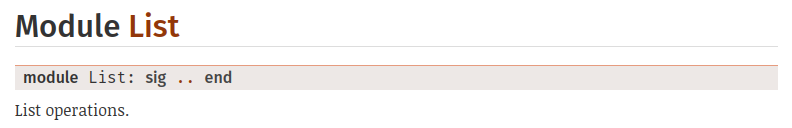
\includegraphics[width=0.8\linewidth]{img/OCaml_List.png}
    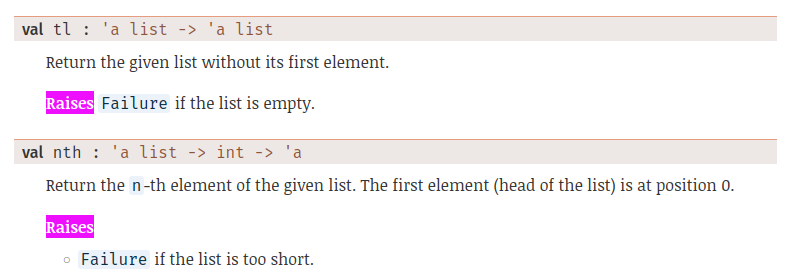
\includegraphics[width=0.8\linewidth]{img/OCaml_List_tl_nth.png}
    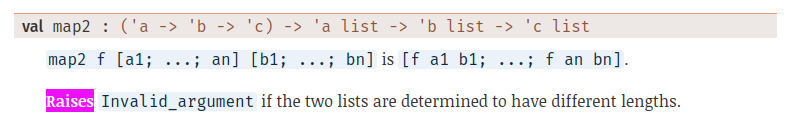
\includegraphics[width=0.8\linewidth]{img/OCaml_List_map2.png}
\end{center}
\end{frame}

\section{Basic Language}

\begin{frame}{Syntax of Types}
\begin{center}
\begin{bnf}
    $A$ : Type ::=
        | $\nat$                 : Natural numbers
        | $\vectype{\ell}$       : Fixed-size list of nats
        | $\pitype{x}{A_1}{A_2}$ : Dependent functions
        ;;
    $\ell$ : Length ::= $n$ // $x$ // $\ell_1 + ... + \ell_k$
        ;;
    $n$ : Numeral :in: $\mathbb{N}$ ;;
\end{bnf}
\end{center}

\begin{block}{Note}
    $A_1 \rightarrow A_2 \triangleq \pitype{\_}{A_1}{A_2}$
\end{block}
\end{frame}

\begin{frame}{Syntax of Terms}
\begin{center}
\begin{bnf}
    $s$ : Syn ::=
        | $x$ // $\app{s}{t}$
        | $\head{\ell}{s}$ // $\tail{\ell}{s}$
        ;;
    $t$ : Chk ::=
        | $s$ // $\lambda x . t$ // $\fix x.t$
        | $n$ // $t_1 + ... + t_k$
        | $\left( \natmatch{s}{t_1}{x}{t_2} \right)$
        | $\nil$ // $\cons{\ell}{t_1}{t_2}$
        | $\left( \vecmatch{s}{t_1}{x_1}{x_2}{x_3}{t_2} \right)$
        ;;
\end{bnf}
\end{center}
\end{frame}

\begin{frame}{Example}
\begin{align*}
    && \texttt{cons} \; &: \; \uncover<2->{\Pi (n \colon \nat) . } \nat \rightarrow \vectype{n} \rightarrow \vectype{(n+1)} \\
    \uncover<3->{
        \textnormal{\deemph{i.e., }}
            && \texttt{cons} \; &: \; \pitype{n}{\nat}{\pitype{\_}{\nat}{\pitype{\_}{\vectype{n}}{\vectype{(n+1)}}}} \\
    }
    \uncover<4->{
        % \textnormal{\deemph{e.g., }}
        %     && [] &\triangleq \nil \\
        \textnormal{\deemph{e.g., }}
            && [10] &\triangleq \cons{{\color{blue} (n = 0)}}{10}{{\color{blue} \nil}} \\
        % \textnormal{\deemph{e.g., }}
        %     && [5, 10] &\triangleq \cons{{\color{blue} (n = 1)}}{5}{{\color{blue} [10]}}
    }
\end{align*}

% \pause

% % TODO: Delete this example to save time?
% \begin{align*}
%     \quad &\texttt{tail} \; : \; \pitype{n}{\nat}{\pitype{\_}{\vectype{(n+1)}}{\vectype{n}}} \\
%     \textnormal{\deemph{i.e., }}
%         \quad &\texttt{tail} \; : \; \pitype{n}{\nat}{\vectype{(n+1)} \rightarrow \vectype{n}} \\
%     \textnormal{\deemph{e.g., }}
%         \quad &\tail{2}{[5, 10, 15]} = [10, 15] \\
%     & \deemph{([5, 10, 15] : \vectype{(2+1)} \textnormal{ and } [10, 15] : \vectype{2})}
% \end{align*}
\end{frame}

\begin{frame}{One More Example}
\begin{align*}
    \textnormal{\deemph{e.g., }} \quad
        & \texttt{drop} \; {\color{darkgreen} (k = 2)} \; {\color{blue} (n = 3)} \; [9, 8, 7, 6, 5] = {\color{blue} [7, 6, 5]}
\end{align*}

\only<-5>{\visible<2->{\alert{Can you spot the mistakes?}}}
\only<6->{{\color{darkgreen} All good now :)}}
\begin{align*}
    & \deemph{\textnormal{// Discard first $k$ elements}} \\
    & \texttt{drop} \; : \; \pitype{k}{\nat}{\pitype{n}{\nat}{\vectype{(k+n)} \rightarrow \vectype{n}}} = \\
        & \qquad \fix{\texttt{drop}} . \lambda k . \lambda n . \lambda v . \\
        & \qquad\qquad \texttt{match} \; k \; \texttt{with} \\
        & \qquad\qquad | \; 0 \rightarrow \only<-2>{\nil}\only<3-3>{\alert{\nil}}\only<4->{{\color{darkgreen} v}}
            \qquad
            \only<3-3>{\textnormal{\alert{$\nil$ does not have type $\vectype{n}$}}}
            \only<4->{{\color{darkgreen} v : \vectype{(0+n)}}} \\
        & \qquad\qquad | \; k' + 1 \rightarrow \texttt{drop} \; \only<-4>{k}\only<5-5>{\alert{k}}\only<6->{{\color{darkgreen} k'}} \; n \; (\texttt{tail} \; (k' + n) \; v) \\
    & \only<5-5>{\alert{\textnormal{$\tail{(k'+n)}{v}$ does not have type $\vectype{(k+n)}$}}}
    \only<6->{{\color{darkgreen} v : \vectype{(k'+1+n)}, \texttt{tail} \; ... : \vectype{(k'+n)}, \texttt{drop} \; ... : \vectype{n}}}
\end{align*}
\end{frame}

\begin{frame}{Judgements}
\begin{columns}
    \begin{column}{0.3\textwidth}
        \widejudgement{$\Gamma \vdash s \syn A$}
    \end{column}
    \begin{column}{0.7\textwidth}
        \vspace{-0.75\baselineskip}
        (In context $\Gamma$, $s$ synthesizes type $A$)
    \end{column}
\end{columns}
\begin{columns}
    \begin{column}{0.3\textwidth}
        \widejudgement{$\Gamma \vdash t \chk A$}
    \end{column}
    \begin{column}{0.7\textwidth}
        \vspace{-0.75\baselineskip}
        (In context $\Gamma$, check that $t$ has type $A$)
    \end{column}
\end{columns}
\begin{columns}
    \begin{column}{0.3\textwidth}
        \widejudgement{$A_1 \equiv A_2$}
    \end{column}
    \begin{column}{0.7\textwidth}
        \vspace{-0.75\baselineskip}
        (Types are equivalent)
    \end{column}
\end{columns}
\begin{columns}
    \begin{column}{0.3\textwidth}
        \widejudgement{$\ell_1 \equiv \ell_2$}
    \end{column}
    \begin{column}{0.7\textwidth}
        \vspace{-0.75\baselineskip}
        (Lengths are equivalent)
    \end{column}
\end{columns}
\end{frame}

\begin{frame}{Rules: Checking}
\smalljudgement{$\Gamma \vdash t \chk A$}

\visible<1->{
    \only<1-2>{
        \begin{inferences}
            \alert<2-2>{
                \infer{\Gamma \vdash \nil \chk \vectype{0}}{}
            }
        \end{inferences}
    }
    \only<-2>{\visible<2->{
        \alert{What about $\Gamma \vdash \nil \chk \vectype{(0 + 0)}$?}
    }}
    \only<3->{
        \begin{inferences}
            \infer{\Gamma \vdash \nil \chk \vectype{\ell}}{\ell \equiv 0}
        \end{inferences}
    }
}
% \visible<4->{
%     \begin{inferences}
%         \infer{
%             \Gamma \vdash \cons{\ell}{t_1}{t_2} \chk \vectype{\ell'}
%         }{
%             \uncover<4->{
%                 \Gamma \vdash \ell \chk \nat
%                 & \Gamma \vdash t_1 \chk \nat
%             }
%             \uncover<4->{
%                 & \Gamma \vdash t_2 \chk \vectype{\ell}
%                 & {\color<4-4>{darkgreen} \ell' \equiv \ell + 1}
%             }
%         }
%     \end{inferences}
% }
\visible<4->{
    \begin{inferences}
        \deduce{
            \infer{
                \Gamma \vdash (\natmatch{x}{t_0}{y}{t_1}) \chk A
            }{
                \uncover<7->{
                    \Gamma' = (\Gamma, y:\nat)
                    & \only<9->{[y+1/x]} \Gamma' \vdash \only<9->{[y+1/x]} t_1 \chk \only<9->{[y+1/x]} A
                }
            }
        }{
            \uncover<5->{\Gamma \vdash x \syn \nat}
            & \uncover<6->{\only<8->{[0/x]} \Gamma \vdash \only<8->{[0/x]} t_0 \chk \only<8->{[0/x]} A}
        }
    \end{inferences}
}
\end{frame}

% TODO: This slide seems a bit crowded
\begin{frame}{Rules: Checking}
\deemph{
    \begin{inferences}
        \deduce{
            \infer{
                \Gamma \vdash (\natmatch{x}{t_0}{y}{t_1}) \chk A
            }{
                \Gamma' = (\Gamma, y:\nat)
                & [y+1/x] \Gamma' \vdash [y+1/x] t_1 \chk [y+1/x] A
            }
        }{
            \Gamma \vdash x \syn \nat
            & [0/x] \Gamma \vdash [0/x] t_0 \chk [0/x] A
        }
    \end{inferences}
}

\begin{align*}
    & \texttt{drop} \; : \; \pitype{k}{\nat}{\pitype{n}{\nat}{\vectype{(k+n)} \rightarrow \vectype{n}}} = \\
        & \qquad \fix{\texttt{drop}} . \lambda k . \lambda n . \lambda v . \\
        & \qquad\qquad \texttt{match} \; k \; \texttt{with} \\
        & \qquad\qquad | \; 0 \rightarrow v
            \qquad
            {\color{darkgreen} v : \vectype{(0+n)}} \\
        & \qquad\qquad | \; k' + 1 \rightarrow \texttt{drop} \; k' \; n \; (\texttt{tail} \; (k' + n) \; v) \\
    & {\color{darkgreen} v : \vectype{(k'+1+n)}, \texttt{tail} \; ... : \vectype{(k'+n)}}
\end{align*}
\end{frame}

\begin{frame}{Rules: Equality}
\smalljudgement{$A_1 \equiv A_2$}
\begin{equation*}
    \begin{cases}
        \nat \equiv \nat \\
        \pitype{x}{A_1}{B_1} \equiv \pitype{x}{A_2}{B_2} & \textnormal{if } A_1 \equiv A_2 \textnormal{ and } B_1 \equiv B_2 \\
        \vectype{\ell_1} \equiv \vectype{\ell_2} & \textnormal{if } \ell_1 \equiv \ell_2
    \end{cases}
\end{equation*}

\uncover<2->{
    \smalljudgement{$\ell_1 \equiv \ell_2$}
    \begin{itemize}
        \item<2-> Normalize and compare syntactically.
        \begin{itemize}
            \item<2-> $1 + n + (2 + m) \longrightarrow 3 + n + m$
            \item<2-> $(n + 0) + 3 + m \longrightarrow 3 + n + m$
        \end{itemize}
    \end{itemize}
}
\end{frame}

\section{Better Pattern Matching}

\begin{frame}{An Unfortunate Restriction}
\begin{itemize}
    \item Subject of \texttt{match} must be a variable $x$ or synthesize $\vectype{x}$
    \begin{itemize}
        \item Needed for substitution
    \end{itemize}
    \item This is why \texttt{head} and \texttt{tail} must be built-in!
\end{itemize}

\begin{align*}
    & \texttt{tail} \; : \; \pitype{n}{\nat}{\vectype{(n+1)} \rightarrow \vectype{n}} = \\
    & \qquad \lambda n . \lambda v . \\
    & \qquad \qquad \texttt{match} \; \alert{v} \; \texttt{with}
        \qquad \alert{v : \vectype{(n+1)}} \\
    & \qquad \qquad | \; \cons{n'}{x}{v'} \rightarrow v' \\
\end{align*}
\end{frame}

\begin{frame}{A Better Approach}
\begin{align*}
    & \texttt{tail} \; : \; \pitype{n}{\nat}{\vectype{(n+1)} \rightarrow \vectype{n}} = \\
    & \qquad \lambda n . \lambda v . \\
    & \qquad \qquad {\color<3-3>{darkgreen} \texttt{match} \; v \; \texttt{with}} \\
    & \qquad \qquad {\color<2-2>{darkgreen} | \; \cons{n'}{\_}{v'} \rightarrow v'} \\
\end{align*}

\visible<2->{
    Is the \texttt{cons} branch correct? (i.e., $\vectype{n} \equiv \vectype{n'}$?)
    \begin{equation*}
        \color<2-2>{darkgreen}
        \forall n, n' \in \mathbb{N} .
            (n' + 1 = n + 1) \implies n = n'
        \qquad \checkmark
    \end{equation*}
}

\visible<3->{
    Is the \texttt{nil} branch unreachable? (i.e., $\vectype{(n + 1)} \not\equiv \vectype{0}$?)
    \begin{equation*}
        \color{darkgreen}
        \lnot\left(
            \exists n \in \mathbb{N} .
                n + 1 = 0
        \right)
        \qquad \checkmark
    \end{equation*}
}
\end{frame}

\begin{frame}{In General}
\begin{itemize}
    \item Add a new context $\Delta ::= \cdot \; | \; \Delta , \ell_1 = \ell_2$
    \begin{itemize}
        \item When entering a \texttt{match}, extend $\Delta$
        \item $\ell \equiv \ell'$ : make a $\forall$ proposition
        \item Reachability : make a $\exists$ proposition
    \end{itemize}
\end{itemize}

\begin{center}
\begin{columns}
    \begin{column}{0.2\linewidth}\end{column}
    \begin{column}{0.25\linewidth}
        \widejudgement{$\Gamma|\Delta \vdash s \syn A$}
        \widejudgement{$\Delta \vdash A_1 \equiv A_2$}
    \end{column}
    \begin{column}{0.25\linewidth}
        \widejudgement{$\Gamma|\Delta \vdash t \chk A$}
        \widejudgement{$\Delta \vdash \ell_1 \equiv \ell_2$}
    \end{column}
    \begin{column}{0.2\linewidth}\end{column}
\end{columns}
\end{center}

\pause

\begin{itemize}
    \item To decide whether propositions are true, use Z3 solver
    \footnote{https://github.com/Z3Prover/z3}
    \item Propositions in Presburger arithmetic are always decidable!
    \footnote{Presburger 1929}
\end{itemize}
\end{frame}

\section{Extending the Language}

\begin{frame}{Booleans}
\begin{itemize}
    \item<1-> Updated syntax:
    \begin{bnf}
        $A$ : Type ::= ... // $\bool$
            ;;
        $t$ : Chk ::=
            | ...
            | $\ttrue$ // $\tfalse$
            | $\left( \boolmatch{s}{t_1}{t_2} \right)$
    \end{bnf}
    \item<2-> New typing rules:
    \begin{inferences}
        \infer{\Gamma|\Delta \vdash \ttrue \chk \bool}{}
        \qquad \infer{\Gamma|\Delta \vdash \tfalse \chk \bool}{}
        \\
        \infer{
            \Gamma|\Delta \vdash (\boolmatch{s}{t_1}{t_2}) \chk A
        }{
            \Gamma|\Delta \vdash s \syn \bool
            & \Gamma|\Delta \vdash t_1 \chk A
            & \Gamma|\Delta \vdash t_2 \chk A
        }
    \end{inferences}
    \item<2-> New case for type equality : $\Delta \vdash \bool \equiv \bool$
    \item<2-> All pretty straightforward!
\end{itemize}
\end{frame}

\section{Conclusion}

\begin{frame}{Limitations}
\begin{itemize}
    \item Vectors can only contain natural numbers
    \begin{itemize}
        \item Can add polymorphism (using Hindley-Milner)
    \end{itemize}
    \item Impossible to implement \texttt{filter}---what should the output length be?
    \begin{itemize}
        \item Can do this using \emph{dependent pairs}
    \end{itemize}
    \item Explicit parameters are not ergonomic
    \begin{itemize}
        \item Could add implicit parameters (as in Agda)
    \end{itemize}
    \item Only addition allowed in lengths
    \begin{itemize}
        \item Cannot implement $\texttt{split}$, $\texttt{join}$, etc.
        % \item Can't really be used as a proof assistant (unlike Agda, Idris, Rocq, etc.)
    \end{itemize}
    % \item Runtime of checking a general proposition in Presburger arithmetic in at least \emph{doubly} exponential
    % \begin{itemize}
    %     \item In practice, the propositions we need to check are not \emph{that} big
    % \end{itemize}
\end{itemize}
\end{frame}

\begin{frame}{Conclusion}
\begin{itemize}
    \item You can check simple constraints on list sizes using dependent types!
    \begin{itemize}
        \item Enforce constraints at compile time
        \item Catch some (but obviously not all) common typos
    \end{itemize}
    \item How to check equivalence of lengths? How to prevent infinite loops in type checker?
    \begin{itemize}
        \item Presburger arithmetic + Z3
    \end{itemize}
\end{itemize}
\end{frame}

\appendix
\section*{Supplemental Slides}

\begin{frame}{Polymorphism}
We implement the Hindley-Milner algorithm.
\begin{center}
\begin{bnf}
    $\hat{A}$ : Type scheme ::= ... &// $\forall\alpha_1, \alpha_2,\dots,\alpha_N.A$
        ;;
    $A$ : Type ::= ... &// $\alpha$
        ;;
    $\Gamma$ : Context ::= $\cdot$ &// $\Gamma , x\colon \hat{A}$
        ;;
    $\sigma$ : Type subst. ::= $\cdot$ &// $\sigma , A/\alpha$
\end{bnf}
\end{center}

\pause

\begin{center}
\begin{inferences}
    \infer{\Gamma \vdash x \syn A}{\Gamma(x) = \hat{A} & \Gamma \vdash \hat{A} \sqsubseteq A}
    \qquad
    \infer{\Gamma \vdash \lambda x.t \chk \pitype{x}{A}{B}}{\Gamma,x:\forall\_.A \vdash t \chk B}
\end{inferences}
\end{center}

\begin{itemize}
    \item Generalization: $\alpha \rightarrow \alpha$ generalizes to $\forall \alpha. \alpha \rightarrow \alpha$.
    \item Instantiation: $\forall \alpha. \alpha \rightarrow \alpha$ can be instantiated to $\nat \rightarrow \nat$.
    \item Unification: $\text{unify}(\alpha \rightarrow \alpha, \nat \rightarrow \nat) = \{\nat/\alpha\}$
\end{itemize}

\end{frame}

% \begin{frame}{A Slight More Involved Example}
% \begin{align*}
%     & \texttt{zip\_with} \; : \; \pitype{n}{\nat}{\vectype{n} \rightarrow \vectype{n} \\
%     & \qquad \qquad \qquad \qquad \rightarrow (\nat \rightarrow \nat \rightarrow \nat) \rightarrow \vectype{n}} = \\
%     & \qquad \fix \texttt{zip\_with} . \lambda n . \lambda v_1 . \lambda v_2 . \lambda f . \\
%     & \qquad\qquad \texttt{match} \; v_1 \; \texttt{with} \\
%     & \qquad\qquad | \; \nil \rightarrow {\color<2-2>{darkgreen} \nil} \\
%     & \qquad\qquad | \; \cons{n'}{x}{v_1'} \rightarrow \\
%     & \qquad\qquad\qquad {\color<4-4>{darkgreen} \texttt{match} \; v_2 \; \texttt{with}} \\
%     & \qquad\qquad\qquad | \; \cons{n''}{y}{v_2'} \rightarrow \\
%     & \qquad\qquad\qquad\qquad {\color<3-3>{darkgreen} \cons{n'}{(f \; x \; y)}{(\texttt{zip\_with} \; n' \; v_1' \; v_2' \; f)}}
% \end{align*}

% \only<2-2>{
%     \color{darkgreen}
%     \begin{equation*}
%         \forall n \in \mathbb{N} . n = 0 \implies n = 0
%         \qquad \checkmark
%     \end{equation*}
% }
% \only<3-3>{
%     \color{darkgreen}
%     \begin{equation*}
%         \forall n, n', n'' \in \mathbb{N} .
%             \left(n = n' + 1 \land n = n'' + 1\right)
%             \implies n' + 1 = n
%         \qquad \checkmark
%     \end{equation*}
% }
% \only<4-4>{
%     \color{darkgreen}
%     \begin{equation*}
%         \lnot \left(
%             \exists n, n' \in \mathbb{N} .
%                 (n = n' + 1) \land (n = 0)
%         \right)
%         \qquad \checkmark
%     \end{equation*}
% }
% \end{frame}

\end{document}
